\documentclass[12pt,english]{article}
\usepackage{setspace}
\doublespacing
\usepackage[affil-it]{authblk}
\usepackage{graphicx}
\usepackage[space]{grffile}
\usepackage{latexsym}
\usepackage{textcomp}
\usepackage{longtable}
\usepackage[flushleft]{threeparttable} 
\usepackage{multirow,booktabs}
\usepackage{ltablex,array} % to scale longtables
\usepackage{lipsum}
\usepackage{amsfonts,amsmath,amssymb}
\usepackage{url}
\usepackage[utf8]{inputenc}
\usepackage{hyperref}
\hypersetup{colorlinks=false,pdfborder={0 0 0}}
\newcommand{\truncateit}[1]{\truncate{0.8\textwidth}{#1}}
\newcommand{\scititle}[1]{\title[\truncateit{#1}]{#1}}
\usepackage[T1]{fontenc}
\usepackage{caption} %have period instead of colon for figures and Table captions
\captionsetup[Table]{labelsep=period}
\usepackage{nopageno}
  
\providecommand{\tabularnewline}{\\}
\usepackage[nolist]{acronym}
\newacro{BMI} {body mass index}  
\newacro{LMIC} {low- and middle-income country}
\acrodefplural{LMIC}[LMICs]{low- and middle-income countries}  
\newacro{MIC} {middle-income country}
\acrodefplural{MIC}[MICs]{middle-income countries}  
\newacro{HIC} {high-income country}  
\acrodefplural{HIC}[HICs]{high-income countries}
\newacro{FE} {fixed effects}  
\newacro{HbA1c} {glycated hemoglobin}  
\newacro{IDF} {International Diabetes Federation}  
\newacro{IV} {instrumental variable}  
\newacro{LPM} {linear probability model}  
\newacro{MxFLS} {Mexican Family Life Survey}  
\newacro{OLS} {ordinary least squares}  
\newacro{RE} {random effects}
\newacro{p.p.} {percentage points}    
\newacro{US} {United States}
\newacro{WHO} {World Health Organization} 
\newacro{USA} {United States of America}   
\usepackage{longtable}
\usepackage{booktabs}
\usepackage{multirow}
\usepackage{graphicx}
\usepackage[Export]{adjustbox}
%landscape pages
\usepackage{pdflscape}
\newcommand{\comment}[1]{}  %allows multiline comments
\usepackage[english]{babel}% Recommended
\usepackage{csquotes}
\usepackage[
maxcitenames=2, 
style=apa,
firstinits=false,
maxbibnames=99,
backend=biber,
uniquename=false,
url=false,
isbn=false,
doi=false]{biblatex}
\DeclareLanguageMapping{english}{english-apa}

\AtEveryBibitem{\clearfield{month}}
	
\addbibresource{/home/till/Dokumente/BibTex/Second_Mexico_paper.bib}

%SPECIFIC FORMATING RULES OF JOURNAL

\renewcommand{\thesection}{\arabic{section}.}
\renewcommand{\thesubsection}{\thesection\arabic{subsection}.}
\renewcommand{\thetable}{\Roman{Table}}




% paper margins
\usepackage{geometry}
\geometry{
letterpaper,
left=25mm,
right=30mm,
top=20mm,
bottom=30mm,
}   
%limiting tables to only float within section
\usepackage{placeins}
  
  
% formating

\usepackage{listings}
\lstset{ %
  backgroundcolor=\color{white},   % choose the background color
  basicstyle=\footnotesize,        % size of fonts used for the code
  breaklines=true,                 % automatic line breaking only at whitespace
  captionpos=b,                    % sets the caption-position to bottom
  commentstyle=\color{OliveGreen},    % comment style
  keywordstyle=\color{BlueViolet},       % keyword style
  stringstyle=\color{black},     % string literal style
  language=[AlLaTeX]TeX,             % Set your language (you can change the language for each code-block optionally)
  frame=lrtb, %
  xleftmargin=\fboxsep, %
  xrightmargin=-\fboxsep, %
  moretexcs={lstset,color,colorlet, cellcolor, newcolumntype, columncolor, rowcolor, multirow, xspace, LaTeX, TeX},
}

	% *****************************************************************
	% siunitx
	% *****************************************************************
\usepackage{siunitx} % centering in tables
\sisetup{
	detect-mode,
	tight-spacing		= true,
	group-digits		= false ,
	input-signs		= ,
	input-symbols		= ( ) [ ] - + *,
	input-open-uncertainty	= ,
	input-close-uncertainty	= ,
	table-align-text-post	= false
}

	        
	        
%For Table commands to change column sizeand alignment, especially tabularx
\newcolumntype{b}{X}  %large columns http://tex.stackexchange.com/questions/84400/Table-layout-with-tabularx-column-widths-502525
\newcolumntype{m}{>{\hsize=.5\hsize}X} % medium columns
\newcommand{\merge}[1]{\multicolumn{2}{>{\hsize=\dimexpr2\hsize+2\tabcolsep+\arrayrulewidth\relax}X}{#1}}  %allows merging of two columns in tabularx http://tex.stackexchange.com/questions/236155/tabularx-and-multicolumn

\newcolumntype{Y}{>{\centering\arraybackslash}X} %new columntype for X columns in tabularx to center them http://tex.stackexchange.com/questions/89166/centering-in-tabularx-and-x-columns
\newcolumntype{Z}{>{\raggedright\let\newline\\\arraybackslash\hspace{0pt}}X} %left aligned X columns http://tex.stackexchange.com/questions/97180/how-to-get-column-alignment-in-tabularx
\newcolumntype{z}{>{\hsize=.5\hsize\\\raggedright\let\newline\\\arraybackslash\hspace{0pt}}X} %left aligned X columns http://tex.stackexchange.com/questions/97180/how-to-get-column-alignment-in-tabularx
\newcolumntype{y}{>{\hsize=.5\hsize}Y} % small columns


        


\makeatletter
\def\@maketitle{%
	\newpage
	\null
	\vskip 2em%
	\begin{center}%
		\let \footnote \thanks
		{\Large\bfseries \@title \par}%
		\vskip 1.5em%
		{\normalsize
			\lineskip .5em%
			\begin{tabular}[t]{c}%
				\@author
			\end{tabular}\par}%
		\vskip 1em%
		{\normalsize \@date}%
	\end{center}%
	\par
	\vskip 1.5em}
\makeatother        

\begin{document}
	\title{The impact of diabetes on labour market outcomes in Mexico: a panel data and biomarker analysis}
	
	\author[a,b]{Till Seuring%
		\thanks{Corresponding author. Leibniz Institute for Prevention Research and Epidemiology - BIPS, Achterstr. 30, 28359 Bremen, Germany, Email: seuring@leibniz-bips.de, Phone: +49 421 218 569 23}}
	\author[b]{Pieter Serneels}
	\author[c]{Marc Suhrcke}
	
	\affil[a]{Leibniz Institute for Prevention Research and Epidemiology - BIPS}
	\affil[b]{University of East Anglia}
	\affil[d]{University of York}
	\date{}	
	
	
	
	\maketitle 
	
	    \noindent Running head: The impact of diabetes on labour market outcomes in Mexico\\
		Keywords: diabetes, employment, wages, biomarker, Mexico, panel data\\
		JEL: I14, I15, J22, J31, D83\\
		Funding statement: No funding was received to support this project.
	\thispagestyle{empty}
	\clearpage
	
\begin{abstract}
There is at best scarce evidence on the economic consequences of diabetes, especially in a context where diabetes often remains undiagnosed, as is the case in low- and middle-income countries. We investigate the impact of diabetes on labour outcomes in Mexico using panel and biomarker data applying fixed effects estimation to account for potential endogeneity and using biomarker information to explore the role of previously undiagnosed diabetes. We find a reduction of 5 percentage points in the probability of being employed for those with self-reported diabetes, in particular in agricultural work, but no impact on wages or hours worked. The employment probability falls gradually with time since diagnosis. In the biomarker analysis we observe that 18\% of all observations are false negatives (undiagnosed), i.e. do not report diabetes but exhibit glycated hemoglobin (HbA1c) levels above the clinical diabetes threshold. The estimated employment impact for those that were found to exceed the threshold (i.e. including those diagnosed with the condition and those undiagnosed) suggests no effects for men but effects for women that are similar compared to self-reported diabetes. Further analysis reveals that there is no effect of diabetes on labour outcomes for undiagnosed women or men. The results highlight both the importance of the economic impact of diabetes, and the need to take into account undiagnosed patients.
\end{abstract}




\section{\label{sec:Introduction4}INTRODUCTION }

Diabetes, a disease characterized by elevated blood glucose levels due to the body's inability to use insulin properly, has become a problem for \acp{LMIC} as well as \acp{HIC}, with over two-thirds of people with diabetes living in the developing world \parencite{InternationalDiabetesFederation2015}. In Mexico, diabetes prevalence is estimated to have grown from 6.7\% in 1994 to 14.4\% in 2006 \parencite{Barquera2013} and 15.8\% in 2015 and diabetes has become the number one contributor to mortality \parencite{InternationalDiabetesFederation2015}, by increasing the risk for heart disease and stroke, blindness, kidney disease and nerve problems, food ulcers and amputations due to elevated glucose levels \parencite{Reynoso-Noveron2011}. However, via effective self-management of the disease much if not all of the complications can be avoided \parencite{Lim2011, Gregg2012}.

The observed trend has been attributed to a deterioration in diet and a reduction in physical activity \parencite{Barquera2008b,Basu2013}, while genetic predisposition among Mexicans with pre-Hispanic ancestry may also play a role \parencite{Williams2013}. The onset of diabetes has been occurring at an ever earlier age in Mexico \parencite{Bello-Chavolla2017a}, which will likely lead to an increase in complications during the productive lifespan, since only a minority of patients in Mexico achieves adequate blood glucose control \parencite{Barquera2013}. Further, the diabetes burden in Mexico coexist with high levels of infectious diseases, exposing the health system to a 'double-disease burden' that increases the pressure to identify treatment priorities and to efficiently use existing resources.

Despite the catastrophic impact of diabetes on health, its economic consequences, in particular in \acp{LMIC} have received less attention, especially its effects on labour outcomes \parencite{Seuring2015a}. The latter have been studied predominantly in high-income countries, suggesting substantial economic losses for individuals and households affected by diabetes \parencite{Brown2005,Brown2014,BrownIII2011,Minor2011,Minor2013,Minor2015,Latif2009}. For \acp{LMIC} less evidence is available. \textcite{Liu2014} exploit a natural experiment in China and find a significant reduction in income due to a recent diabetes diagnosis. A study for Mexico using cross-sectional data from 2005, finds a significant (p<0.01) reduction in employment probabilities for males by 10 \ac{p.p.} and for females by 4.5 \ac{p.p.} (p<0.1) \parencite{Seuring2015}. So far, most studies have relied on an \ac{IV} strategy that uses the genetic component of diabetes based on its family history as an instrument, to address the potential endogeneity of diabetes.  However, family history of diabetes may also proxy for other genetically transferred traits, including unobserved abilities, as well as  intrahousehold or intergenerational dynamics that impact labour outcomes directly; the validity of this \ac{IV} strategy remains therefore debatable. Panel data methods to account for time-invariant unobserved individual characteristics, haven not yet been used. Time-invariant unobservables such as health endowments or risk preferences could adversely affect health in general and the propensity to develop type 2 diabetes in particular \parencite{VanEwijk2011,Sotomayor2013,Li2010b}; they may also affect labour outcomes---either directly through their effects on contemporaneous productivity \parencite{Currie2013}, or indirectly by limiting educational attainment and human capital accumulation \parencite{Ayyagari2011a}. These unobservables thereby present a major source of a potential bias that could be accounted for by the use of individual \ac{FE}, which does not rely on the strong assumptions of an \ac{IV}.


Other limitations of the previous literature include only limited evidence on the severity of the potential labour market penalties over the duration of diabetes. Further, undiagnosed diabetes---a particular problem in \acp{LMIC} \parencite{Beagley2014}---has mostly remained unaccounted for, ignoring potential differences between those with diagnosed and undiagnosed diabetes. These could be caused by stress, depression or anxiety resulting from a diagnosis \parencite{Liu2014}, or by the disease being used to justify reduced labour supply \parencite{Kapteyn2009}. Further, a diabetes diagnosis may often be related to the transition from an asymptotic to symptomatic state with the  appearance of complications, leading to a selection of people in worse health and at a later diabetes stage into the diagnosed/self-reporting population. Similarly, a diagnosis may also be related to socioeconomic factors affecting the access to health care and its quality, leading to a selection of better educated and wealthier individuals into the diagnosed population.

The objective of this study is to provide new evidence on the impact of diabetes on labour outcomes, adding to previous work by paying close attention to the challenges of unobserved heterogeneity, to the chronic nature of diabetes and to the population unaware of their condition (i.e. the 'undiagnosed'). We use three waves of Mexican panel data, covering the period 2002--2012. Applying individual level fixed effects, we take account of time-invariant heterogeneity when assessing the impact of self-reported diabetes and of time since diagnosis on labour outcomes.\footnote{A recent review of the economic cost of diabetes confirms the scarcity of evidence for low- and middle-income countries \parencite{Seuring2015a}.} We also make use of rich and novel biomarker data from the most recent wave of data, to explore the role of undiagnosed diabetes.

\section{\label{sec:Data}DATA}

This paper uses the \acf{MxFLS}, a nationally representative longitudinal household survey containing three waves conducted in 2002, 2005--2006 and 2009--2012. It collects data on a wide range of social, demographic, economic and health characteristics \parencite{Rubalcava2013}. The samples used are restricted to the working age population (15--64). The first part of the analysis uses all three waves and the panel structure of the data. The second part uses a biomarker subsample of the third wave (2009--2012). Because the biomarker sample includes everybody above the age of 44 but only a random subsample of those aged 44 or below \parencite{Crimmins2015}, its age structure is older and hence its self-reported diabetes prevalence is higher. This reduces direct comparability to the panel results and biomarker based results will be compared to the analysis of the self-reported data for this specific subsample.

Our outcome variables are employment status, hourly wage, weekly working hours and occupation.\footnote{Employment status is defined as having carried out an activity that helped with the household expenses the last week and working for at least four hours per week. We explicitly include informal employment, for instance in family business. Changing the definition to having worked at least ten hours per week only leads to marginal changes in the results, and does not affect the interpretation.  Hourly wage is constructed as reported monthly income from the first and second job, divided by average number of weeks per month and weekly working hours.  Labour income is obtained from the response to questions on wages, income from piecework, tips, income from extra hours, meals, housing, transport, medical benefits and other earnings, or from the response to a question on aggregate labour income for the entire month. We adjusted calculated wages for inflation in the year of interview and consider the log of real wages. Due to a considerable number of missing or zero income reports, the sample used for the wage estimation is smaller than the sample for working hours. Working hours are for both the first and second job.} Descriptive statistics for the entire panel sample show that 86\% of men report some form of employment compared to 37\% of women (see Table \ref{tab:Pooled-sample-characteristics}). Interestingly, men do not report considerably higher hourly wages than women but work more hours per week. Men also work more often in agricultural jobs while women are more likely to be self-employed or in non-agricultural wage employment. The educational attainment of women is lower than that for men on average.

The first part of the analysis focuses on the relationship of labour outcomes with self-reported diabetes\footnote{Self-reported diabetes is based on the survey question: “Have you ever been diagnosed with diabetes?”}. For the pooled data of all three waves (Table \ref{tab:Pooled-sample-characteristics}), diabetes was self-reported by 5\% of men and 6\% of women, respectively. This is consistent with \textcite{Barquera2013}, who observe a prevalence of diagnosed diabetes in Mexico of 7.5\% in 2006, using a slightly older sample that also included respondents beyond 64 years of age. Apart from self-reported diabetes information that is available in all rounds, we also use information on the self-reported year of diagnosis as well as biometrically measured \ac{HbA1c} levels for a subsample of respondents. Throughout, our analysis focuses on the working age population (15--64), and exclude pregnant women and those in school.\footnote{Pregnant women have an increased diabetes risk and this may bias the estimated impact of diabetes on female employment status. We dropped all observations of women reporting to be pregnant at the time of the survey (N=764). Considering the entire sample and including a dummy for pregnant women only leads to minor changes in the results and does not affect the interpretation.}

\begin{center}
	\textbf{Table \ref{tab:Pooled-sample-characteristics} about here}
\end{center}

Because the self-reported diabetes data exhibited some inconsistency over time for some of the respondents, we apply corrections using disease information from earlier and subsequent waves to infer the current (missing or inconsistent) diabetes status.  Appendix A provides details on the procedure. Information on the self-reported year of diagnosis allows us to construct a measure of time since diagnosis.  Since the timing of diagnosis was only asked in the third wave, this limits the sample to those that were present in the third wave only (but still allows allows panel data analysis).

The second part of the analysis assesses the role of measurement error associated with self-reported diabetes by also considering those with undiagnosed diabetes, i.e. the false negatives. These are identified by their biometrically measured blood glucose value, which is available for over 6000 respondents in the third wave and allows us to test for  differences between the effects of self-reported and undiagnosed diabetes on labour outcomes.

Summary statistics for the biomarker data indicate that a large share of the sample (27\%) have an \ac{HbA1c} indicative of diabetes (Table \ref{tab:Pooled-sample-characteristics}), defined as levels equal to or above 6.5\% \parencite{WorldHealthOrganization2011}, and a large proportion of the sample (18\%) are false negatives, implying that 68\% of males and females who test positive do not self-report and hence are unaware of their condition.




%\FloatBarrier

\section{\label{sec:Estimation Strategy}ESTIMATION STRATEGY}

To investigate the relationship between self-reported diabetes and three labour outcomes---employment, wages and weekly working hours---we estimate the following \acf{FE} model.\footnote{We do not present the random effects results as the Hausman test suggested the use of the \ac{FE} model throughout; they are available upon request.}


\begin{equation}
Y_{it}=\beta_{0}+\beta_{1}Diabetes_{it}+\beta_{2}X_{it}+c_{i}+\gamma_{t}+u_{it}.\label{eq:cha4_employed}
\end{equation}


where $Y_{it}$ is a binary variable taking a value of $1$ if respondent $i$ reports being in employment at time $t$ and $0$ otherwise, $Diabetes_{it}$ is a binary variable taking a value of $1$ at time $t$ if the respondent reports having ever received a diagnosis of diabetes\footnote{The data at hand does not allow distinguishing between type 1 and type 2 diabetes. Existing studies find no effect of type 1 diabetes on labour outcomes  \parencite{Minor2011,Minor2015}. Our estimates of type 2 diabetes impact on labour outcomes may therefore be attenuated and can be seen as providing a lower bound.}, $X_{it}$ is a vector of control variables, $c_{i}$ represents an individual fixed effect, $\gamma_{t}$ represents year dummies, while $u_{it}$ captures the error term.

For the relationship of diabetes with wages and working hours, our empirical models are estimated conditional on being in employment. $Y_{it}$ represents the log hourly wage or the weekly working hours over the last year, for respondent $i$ at time $t$.

The regressions control for level of urbanization, education, state, marital status, the number of children below the age of 6  in the household, a quadratic age term, calendar year dummies as well as household wealth.\footnote{We compose an indicator using principal component of household assets and housing following \textcite{Filmer2001}. The assets indicators reflect owning a vehicle, a second house, a washing machine, dryer, stove, refrigerator or furniture, any electric appliances, any domestic appliances, a bicycle, farm animals, and accounts for the physical condition of the house, proxied by the type of floor material and water access.}. 

Importantly, omitted time-variant variables and simultaneity may still affect the relationship of interest when using a \ac{FE} model. For instance, job loss might lead to lifestyle choices that cause changes in the probability to develop diabetes, which could in turn affect labour outcomes. While we cannot exclude this possibility, existing work for high-income countries finds no evidence for this type of reverse causality \parencite{Bergemann2011,Schaller2015}, suggesting that the \ac{FE} approach will help considerably in reducing  bias.


\subsection{Labour outcomes and time since diagnosis}

The chronic nature and irreversibility of diabetes provide good reason to explore the long term effects post diagnosis.  We estimate the following model:

\begin{equation}
Y_{it}=\beta_{0}+\beta_{1}Dyears_{it}+\beta_{2}X_{it}+c_{i}+u_{it},\label{eq:duration_linear}
\end{equation}

where $\beta_{1}Dyears_{it}$ is continuous indicating years since the diagnosis was first reported.\footnote{Note that while simultaneous inclusion of year dummies and time since diagnosis (which varies by one unit in each time period) would typically not allow separate identification of the coefficient of time since diagnosis in Eq. \ref{eq:duration_linear} and Eq.  \ref{eq:splines}, identification here relies on the presence of people without diabetes in the sample, for which diabetes duration does not increase.  Models excluding the calendar year dummies provide similar results.  As a further robustness check, we estimate two models that only use between-individuals variation, i.e. a \ac{LPM} that uses only data from the third wave, the only wave where year of diagnosis was originally reported, and a pooled \ac{LPM} that used data from all three waves. The results remain the same.} We also consider a spline function that allows for non-linear effects over time.

\begin{equation}
Y_{it}=\delta_{0}+g(Dyears_{it})+\delta_{2}X_{it}+c_{i}+u_{it}.\label{eq:splines}
\end{equation}

\noindent with $g(Dyears_{it})=\sum_{n=1}^{N}\delta_{n}\cdot max\{Dyears_{it}-\eta_{n-1}\}I_{in}$ and $I_{in}=1[\eta_{n-1}\leq Dyears_{it}<\eta_{n}]$, with $\eta_{n}$ being the place of the $n$-th node for $n=1,2,\ldots,N$. The coefficient $\delta_{n}$ captures the effect of diabetes for the $n$-th interval. The effects are linear if $\delta_{1}=\delta_{2}=,\ldots,=\delta_{n}$.\footnote{Because the year of diagnosis was only reported in the third wave, time since diagnosis is not available for those who were not interviewed in the third round.  A reported diagnosis in the year of the interview is counted as 'one year since diagnosis'.} Based on visual inspection (Figure \ref{fig:Kernel-weighted-local-polynomial_comb} on page \pageref{fig:Kernel-weighted-local-polynomial_comb}) we choose three nodes located at 4, 11 and 20 years after diagnosis. The first four years capture any immediate effects of the diagnosis, the years five to eleven any effects during time of adaptation to the disease and the last term (beyond 11 years) accounts for the long-term effects.

\subsection{\label{sec:Biomarker Strategy}Labour outcomes and biometrically measured diabetes}

The analysis consists of three steps. We first re-estimate Eq. \ref{eq:diab_sr} to assess the relationship between self-reported diabetes with labour outcomes, but this time for the cross-sectional biomarker sample only, using the following specification:
\begin{equation}
Y_{i}=\beta_{0}+\beta_{1}Dsr_{i}+\beta_{2}X_{i}+c_{i}+v_{i}\label{eq:diab_sr}
\end{equation}

where $v_{i}$ are community fixed effects which reflect local unobserved characteristics such as access to healthcare, poverty and unemployment in the community.\footnote{We did not use household fixed effects since the average number of observations per household was close to one, as most households had only one member providing biomarker information.}

In a second step we then estimate the relations between biomarker diabetes and labour outcomes, using the following equation:

\begin{equation}
Y_{i}=\beta_{0}+\beta_{1}Dbio^{d}_{i}+\beta_{2}X_{i}+v_{i}+u_{i}\label{eq:diab},
\end{equation}

where $Dbio^{d}$ is equal to $1$ if \ac{HbA1c} $\geq6.5\%$. 

To estimate the effect of undiagnosed diabetes, we add self-reported diabetes back in and interact it with the biomarker in Eq. \ref{eq:diab_ud}.

\begin{equation}
Y_{i}=\beta_{0}+\beta_{1}Dsr_{i}+\beta_{2}Dbio_{i}+\beta_{3}Dsr_{i}*Dbio_{i}+\beta_{4}X_{i}+v_{i}+u_{i}.\label{eq:diab_ud}
\end{equation}

The interaction term changes the interpretation of $\beta_{1}$ and $\beta_{2}$, with $\beta_{1}$ now representing the effect on those aware of their condition but with \ac{HbA1c} levels below the diabetes threshold; $\beta_{2}$ measures the effect on those with undiagnosed diabetes, i.e. the respondents not self-reporting diabetes but with \ac{HbA1c} levels equal to or above the threshold. The interaction term $\beta_{3}$ shows the effect for those with self-reported diabetes and \ac{HbA1c} levels above the threshold. We then test if $\beta_{1} + \beta_{3} = \beta_{2}$, i.e. if the effect of self-reported diabetes is significantly different from that of undiagnosed diabetes.

We further investigate the effect of the severity of diabetes on labour outcomes, replacing $Dbio^{d}$ with $Dbio^{c}$ , a variable that is 0 for \ac{HbA1c} < 6.5\% and takes the actual value of \ac{HbA1c} for those with an $HbA1c \geq 6.5\%$ (Eq. \ref{eq:diab_hba1c}). This will allow us to investigate the effect of a one percentage point increase in \ac{HbA1c} levels for people with undiagnosed diabetes ($\beta_{2}$) as well as for those with self-reported diabetes above the diabetes threshold ($\beta_{3}$).

\begin{equation}
Y_{i}=\beta_{0}+\beta_{1}Dsr_{i}+\beta_{2}Dbio^{c}_{i}+\beta_{3}Dsr_{i}*HbA1c_{i}+\beta_{4}X_{i}+v_{i}+u_{i}.\label{eq:diab_hba1c}
\end{equation}

\section{\label{sec:cha_4_results}RESULTS}


\subsection{Labour outcomes and self-reported diabetes}

The results of estimating Eq. \ref{eq:cha4_employed} in Table \ref{tab:Self-reported-diabetes-and} indicate significant and substantial reductions in the probability of employment for men and women with self-reported diabetes. Employment probabilities are reduced by over 5 \ac{p.p.} for both genders, translating into relative reductions of 14\% for women and of 6\% for men. There is no significant relationship between wages and working hours (Columns 3--6 of Table \ref{tab:Self-reported-diabetes-and}).

Since  wages and working hours may be affected differently depending on the  physical demands in different work types, we interact diabetes with agricultural employment and self- employment, using non-agricultural wage employment as the comparison group (Table \ref{tab:Self-reported-diabetes-and} panel B). However, while the interaction term for diabetes on work hours in agriculture indicates a reduction compared to non-agricultural employment, the Wald test does not indicate a significant difference to agricultural workers without diabetes  ($p = .15$), indicating no effect when stratifying by worktype.

\begin{center}
	\textbf{Table \ref{tab:Self-reported-diabetes-and} about here}
\end{center}

The lack of effects at the internal margin may be explained by selection bias, with those with 'mild' or asymptomatic diabetes being more likely to maintain their productivity. Only once complications become increasingly severe would they switch activity, or stop supplying labour.

To assess whether diabetes affects the selection into different types of work, we assess the role of diabetes for the probability of being in non-agricultural wage employment, agricultural employment or self-employment, using \ac{FE} models.  We only find evidence for negative effects on the probability to work in agriculture for women, possibly due to  relatively higher physical requirements (Table (\ref{tab:Self-reported-diabetes-selection_LPM}).\footnote{We prefer this model to a multinomial logit because it allows individual level fixed effects; it also produces results that are straightforward to interpret. As a robustness check we estimated a multinomial logit model that includes means of time-varying covariates to proxy for fixed effects (see \textcite{Mundlak1978,Bell2015}), and this yields very similar results, both in size and statistical significance.}

\begin{center}
	\textbf{Table \ref{tab:Self-reported-diabetes-selection_LPM} about here}
\end{center}

\subsection{\label{sec:duration}Labour outcomes and time since diagnosis}

Figure \ref{fig:Kernel-weighted-local-polynomial_comb} shows that the probability of employment for men steadily declines as time progresses, using non-parametric kernel-weighted local polynomial regression. For women, a first drop-off occurs right after diagnosis; followed by no consistent pattern thereafter.\footnote{Since long run estimations suffer from large standard errors---as the sample size is strongly reduced---this limits its interpretation and we therefore truncate the graphs at a disease duration of 24 years.} The dynamics for wages and working hours are less clear, with a possibly long term negative trend for women but not for men.

\begin{center}
	\textbf{Figure \ref{fig:Kernel-weighted-local-polynomial_comb} about here}
\end{center}


Table \ref{tab:Self-reported-diabetes-duration_employ} panel A shows the results of estimating Eq. \ref{eq:duration_linear}, which indicate that male employment probabilities fall every year, with the biggest effects being observed in the \ac{FE} model. For women, the coefficient shows a reduction of close to 1 percentage point per year in the \ac{FE} model.



\begin{center}
	\textbf{Table \ref{tab:Self-reported-diabetes-duration_employ} about here}
\end{center}


Panel B shows the estimates of using a spline function as described in Eq. \ref{eq:splines}, providing some evidence for an immediate effect of diabetes on men employment probabilities, which then levels off for some time after which it becomes stronger again.

Female wages are reduced by about 7\% per year after diagnosis in the linear \ac{FE} model, while no effect is found for men. The non-linear results suggest that wages are reduced 5--11 years after the initial diagnosis for both men and women, and potentially after more than 20 years for women only.\footnote{The results for over 20 years may be fragile as they stem from a low number of observations There are only 9 (3) observations for male (female) wages with more than 20 years since diagnosis in wave 3, and 17 (7) in the pooled sample. For male (female) working hours there are 12 (7) observations with more than 20 years since diagnosis in wave 3, and 20 (12) for the pooled sample.}


\FloatBarrier

\subsection{Cross-sectional biomarker analysis}


Table \ref{tab:Biomarker_observations} presents a cross tabulation of self-reported diabetes and biomarker results. Overall, for 80\% of the observations the self-reports are consistent with the biomarker results (diagonal cell \%), 18\% are false negatives or undiagnosed and 2\% false positives, though the latter may include cases that received a diabetes diagnosis and managed to reduce their \ac{HbA1c} to non-diabetes levels via medication and/or lifestyle changes \parencite{Flores-Hernandez2015}. There are no considerable differences between men and women.\footnote{Results available on request.}

\begin{center}
	\textbf{Table \ref{tab:Biomarker_observations} about here}
\end{center}


Table \ref{tab:Biomarker_results} presents the results from estimating Eq. \ref{eq:diab_sr} -- \ref{eq:diab_hba1c}. Panel A confirms the earlier longitudinal results using self-reported diabetes carry for the cross-sectional biomarker sample. The results in panel B indicate that the relationship with employment becomes weaker when using diabetes defined by the biomarker instead of self-reported diabetes, in particular for men. Results in Panel C are obtained from estimating Eq. \ref{eq:diab_ud} and indicate an absence of a (statistically significant) negative relationship between undiagnosed diabetes (expressed in the 'Biomarker diabetes but not self-reported' coefficient) and labour outcomes. The coefficients for the interaction term are negative throughout, though only statistically significant for male wages and female working hours. The F-test shows little evidence for a difference between self-reported diabetes ($\beta_{1} + \beta{3}$) and undiagnosed diabetes ($\beta_{2}$), apart from female working hours and potentially male employment probabilities.

\begin{center}
	\textbf{Table \ref{tab:Biomarker_results} about here}
\end{center}


To explore whether the adverse effects increase with higher  \ac{HbA1c} levels we estimate Eq. \ref{eq:diab_hba1c}. The results in panel D support the findings from panel C, showing negative coefficients for a 1 percentage point increase in \ac{HbA1c} for those with self-reported diabetes and \ac{HbA1c} levels in the diabetes range, again, however, only statistically significant for male wages and female working hours. For undiagnosed diabetes, we find again no effects.

To further understand the smaller impact of undiagnosed diabetes, we next examine potential mediators. First, we include a range of indicators for other chronic diseases that are often related to diabetes: being overweight or obese (based on anthropometric measures of \acf{BMI}) and self-reported hypertension and heart disease. If those diagnosed with diabetes are more likely to experience adverse labour outcomes because they are more likely to suffer from one of these conditions, then accounting for them should lead to a reduction in the coefficient of self-reported diabetes. Panel A of Table \ref{tab:Diagnosed_undiagnosed_condensed}, however, indicates only small reductions in the coefficients of self-reported diabetes ($\beta_{1}+\beta_{3}$), suggesting no major contributions of these factors to the economic burden of diabetes. 

\begin{center}
	\textbf{Table \ref{tab:Diagnosed_undiagnosed_condensed} about here}
\end{center}

Controlling for subjective health instead of chronic diseases, the results reported in Table \ref{tab:Diagnosed_undiagnosed_condensed}, panel B, show a more notable change in coefficients. The overall effect of self-reported diabetes on the probability of male employment is now comparatively smaller and becomes statistically insignificant. The effect of undiagnosed diabetes in men remains close to zero. For women, the coefficient for self-reported diabetes is also reduced, while the effect of undiagnosed diabetes remains the same. We do not observe major changes for any of the other outcomes.   






\section{\label{sec:cha_4_conclusion}DISCUSSION}

Diabetes is now one of the most common chronic diseases in low- and middle as well as high-income countries, with the potential to severely impact the health and economic well-being of those affected.  Yet rigorous evidence on the economic consequences for \acp{LMIC} remains scarce.

To address key methodological challenges, this paper uses rich longitudinal panel data from Mexico that also contain diabetes biomarker. The biomarker data confirm the alarming levels of clinically tested diabetes (27\% prevalence) and indicate that a large proportion of the population (18\%) is unaware of their condition.

Overall, the paper finds evidence for adverse effects of self-reported diabetes on the probability of being employed,  using fixed effects estimation, confirming earlier findings for Mexico regarding the employment impact of diabetes that used cross-sectional information. Nonetheless, these new results also suggest a comparatively larger impact of diabetes on female employment probabilities. Analysis of the long term impact suggests that the employment probability falls gradually over the years after having been diagnosed. This contrasts with estimates for the USA \parencite{Minor2013}, where reductions in employment probabilities only fell after 11 to 15 years for females and after 2-5 years for males.\footnote{Note that the non-linear results are not directly comparable to those from  \textcite{Minor2013} who used pooled cross-sectional data, made use of dummy variables to indicate time since diagnosis, and used different categories of duration.   When we follow the same approach as  \textcite{Minor2013}, we find a significant reduction in employment probabilities throughout.} 

For wages and working hours the results are more ambiguous, and only specifications taking into account the time since diagnosis indicate an adverse relationship. Interestingly, the reductions in wages in the non-linear analysis of time since diagnosis appear at the time where employment probabilities remain unaffected, suggesting that reductions in productivity translate into lower wages but not job loss. Considering different types of work, the relationship between self-reported diabetes, wages and hours worked remains weak, but the results also suggest occupational selection with women with self-reported diabetes less likely to work in agriculture. 

Making use of the biomarker data we find that diabetes based on biomarkers is less related to reduced employment compared to self-reported diabetes, in particular for men. Further analysis shows that this is due to the non-relationship between undiagnosed diabetes and employment.  For the USA, \textcite{Minor2015}  find---similar to us---no statistically significant effects of undiagnosed diabetes on employment, while the effect of diagnosed diabetes is significant. Our results further suggest, that the  difference  in the employment impact of diagnosed and undiagnosed diabetes is not mediated by current \ac{HbA1c} levels, but rather overall health status. This is supported by findings for Mexican-Americans in the USA, where employment outcomes were found to be lower for those with increased \ac{HbA1c} levels \parencite{BrownIII2011}. This may not be surprising given that \ac{HbA1c} levels are only informative for the last three months, and are not the only indicator for the severity of diabetes. \ac{HbA1c} levels may further be affected by treatment, so that people with already severe diabetes complications and a long diabetes duration may have lower levels due to their medical treatment and experience with managing the disease. 

Our findings bear several implications.  First, the impact of self-reported diabetes on labor outcomes in Mexico is mostly limited to its effect on employment probabilities, though there is some indication that it could also reduce wages over time, in particular in the intermediate time after diagnosis where complications are still less severe.  Second, its effect on employment is much stronger for females.  The underlying reasons remain unclear. Potential explanations are that lower wages or working hours for women make a dropout less costly, or discriminate against women with diabetes may be easier. Other evidence suggests that  women with diabetes are in worse metabolic health compared to men when they cross the diabetes threshold \parencite{Peters2015}. Third, one cannot assume that estimates based on self-reported diabetes extend to those with undiagnosed diabetes. Studies should therefore, whenever possible, account for both groups separately, acknowledging their inherent differences, to gain information about the distribution of the economic burden in the diabetes population.

Our results add further weight to the case for reducing the incidence and progression of diabetes.   The large proportion of previously undiagnosed cases indicates that diagnosis---at least in Mexico---happens too late or not at all. This reduces the possibilities to prevent complications via treatment and self-management, increasing the risk of severe complications to appear earlier. Earlier diagnosis and ensuing effective treatment may lighten the health and economic burden. Further, there is a  need to explore why women experience such strong economic effects.  Ultimately, prevention of diabetes is of high importance. Taxation of sugar sweetened beverages may be one promising way forward \parencite{Colchero2016}, though their long-term effectiveness remains unclear. Therefore, addressing the double-disease burden of non-communicable and communicable diseases via investments in maternal and child health may be particularly promising, in particular given the established links between early life heath and later life incidence of diabetes and other chronic diseases \parencite{Sotomayor2013,Hanson2012,Li2010b}.



\clearpage
\begin{appendix}



\part*{\label{part:Appendix}Appendix}

\section{\label{sec:Appendix}Strategies to deal with inconsistent self-reporting over time}

Reporting error can pose a considerable challenge in the use of self-reported data. Fortunately, the \ac{MxFLS} data provide several possibilities to assess the amount of misreporting and apply corrections before estimating the labour market effects of diabetes. In what follows we describe how we have dealt with inconsistencies in self-reported diabetes over time.

Throughout the surveys, self-reported diabetes was measured by the question 'Have you ever been diagnosed by diabetes'. If they answered 'yes', they were asked if they received treatment for diabetes and the type of treatment they received.

One of the key advantages of panel data is the repeated measurement which results in more than one data point allowing to uncover inconsistencies for cases with multiple observations. Very little is known about inconsistencies in self-reported diabetes over time. However, \textcite{Zajacova2010} assess the consistency of a self-reported cancer diagnosis over time in the USA. The study found that 30\% of those who had reported a cancer diagnosis at an earlier point failed to report the diagnosis at a later point in time. A more recent diagnosis was found to be reported with greater consistency possibly due to increasing recall problems as time since diagnosis advanced.

When assessing the \ac{MxFLS}, we also found inconsistencies in the diabetes self-reports across the three waves, with between 10--20\% of those reporting diabetes in one wave not doing so in one of the subsequent waves. To improve the validity of diabetes self-reports, we were interested in reducing the amount of reporting inconsistencies.

As discussed at the end of section \ref{sec:Data}, for diabetes, the main concern with mismeasurement is related to false negatives. False positives are deemed less of a problem since incentives to report diabetes when one does not have it seem to be very limited---although we cannot exclude this.  A study from China finds that the vast majority (98\%) of those who self-report diabetes are tested positive for diabetes, while only a minority  of those who are tested positive for diabetes (40\%) actually self-report the disease \parencite{Yuan2015}.  Our data showed a similar pattern, with a negligible proportion (3\%) of the respondents who are tested negative self-reporting to suffer from diabetes, while the majority of those who are tested positive (68\%) do not self-report suffering from diabetes.

We used the above information to infer the "true" diabetes status for those with inconsistent reports. For respondents present in all three waves, we corrected inconsistencies as reported in Table \ref{tab:Inconsistencies}. We assumed that if diabetes was reported only once in the first two waves (either in 2002 or 2005) and then not reported again in the ensuing waves, this diabetes report was likely to be false (see lines 3 and 4 in Table \ref{tab:Inconsistencies}) and that the person never had received a diagnosis. If a diabetes diagnosis was however reported in two of the three waves (in 2002 and 2009 but not 2005, or in 2002 and 2005 but not in 2009) we assumed that the respondent had diabetes in all three waves (see lines 1 and 2 in Table \ref{tab:Inconsistencies}). For cases where we only had information from two waves, we assumed that if a diabetes diagnosis had been reported in a prior wave they also had diabetes in the ensuing wave, even if it was not reported in the latter (see lines 5 and 6 in Table \ref{tab:Inconsistencies}), given that most diabetes self-reports tend to be correct.


\begin{center}
	\textbf{Table \ref{tab:Inconsistencies} about here}
\end{center}




We then tested if those respondents we categorized as not having a diabetes diagnosis based on above rules were actually more likely to not have diabetes, using the biomarker data from wave 3. Of those with inconsistencies in their diabetes self-reports, 95 were present in the biomarker sample (46 with two self-reports (from lines 3 and 4 in Table \ref{tab:Inconsistencies}) and 49 with one self-report of diabetes (from lines 1 and 2 in Table \ref{tab:Inconsistencies})). Figure \ref{fig:kdens_inconsistency_hba1c} illustrates the difference between both groups and suggests that indeed those with two self-reports of diabetes are much more likely to have \ac{HbA1c} values above the diabetes threshold. A t-test comparing the mean \ac{HbA1c} for the two groups indicates that those with two self-reports also have significantly (p<0.001) higher \ac{HbA1c} levels than those with only one self-report of diabetes (9.7\% vs. 7.1\%). Further, of those with one self-report,  only 30\% have an \ac{HbA1c}$\geq6.5$\% compared to 87\% of those with two self-reports. Based on these results it appears that we did minimize misclassification of people into diabetes or no-diabetes. 

Alternatively we also test if using an alternative strategy, i.e. assuming that everybody who reported  a diabetes diagnosis once had diabetes in any later wave, would lead to different estimation results. We do not find this to be the case and find only minor differences in the point estimates of the coefficients (results available on request). 

\begin{center}
	\textbf{Figure \ref{fig:kdens_inconsistency_hba1c} about here}
\end{center}


\section{\label{sec:Appendix_B}Studies on diabetes and labour market outcomes}
\begin{center}
	\textbf{Table \ref{tab:rev_Diab_employment} about here}
\end{center}



\end{appendix}




\printbibliography




\begin{table}[p]
	\caption{\label{tab:Pooled-sample-characteristics}Descriptive statistics for panel and biomarker sample.}
	
	\begin{adjustbox}{max width=0.7\linewidth, center}
		\begin{threepartTable}  %adds notes to tables
			{
				\def\sym#1{\ifmmode^{#1}\else\(^{#1}\)\fi}
				\begin{tabular}{l*{4}{SS}}
					\toprule
					&\multicolumn{2}{c}{Panel}&\multicolumn{2}{c}{Biomarker}\\\cmidrule(lr){2-3}\cmidrule(lr){4-5}
					&\multicolumn{1}{c}{Males}&\multicolumn{1}{c}{Females}&\multicolumn{1}{c}{Males}&\multicolumn{1}{c}{Females}\\
					\midrule
					\hspace*{10mm}\emph{Dependent variables} \\
					Employed           &        0.86&        0.37&        0.86&        0.34\\
					&      (0.34)&      (0.48)&      (0.35)&      (0.47)\\
					Hourly wage (Mexican Peso)        &      42.47&       40.49&       36.30&       35.23\\
					&    (485.87)&    (142.08)&     (53.69)&     (43.63)\\
					Weekly working hours&      46.82&       38.99&       46.00&       38.15\\
					&     (16.79)&     (18.90)&     (16.89)&     (19.65)\\
					Agricultural worker &        0.22&        0.04&        0.25&        0.03\\
					&      (0.41)&      (0.20)&      (0.43)&      (0.18)\\
					Self-employed       &        0.19&        0.28&        0.21&        0.32\\
					&      (0.39)&      (0.45)&      (0.41)&      (0.47)\\
					Non-agricultural worker &&&&\\
					or employee& 0.59&        0.68&        0.53&        0.64\\
					&      (0.49)&      (0.47)&      (0.50)&      (0.48)\\
					\hspace*{10mm}\emph{Diabetes variables} \\
					Self-reported diabetes  &         0.05&        0.06&        0.09&        0.12\\
					&      (0.22)&      (0.24)&      (0.29)&      (0.32)\\
					Diabetes duration if self- &&&&\\
					reported diabetes (years)   &        7.49&        7.83&        7.48&        7.99\\
					&      (6.01)&      (7.83)&      (6.07)&      (7.03)\\
					Glycated hemoglobin (HbA1c)&            &            &       6.46&        6.58\\
					&            &            &      (1.89)&      (2.02)\\
					HbA1c $\geq 6.5\%$  &            &            &        0.26&        0.28\\
					&            &            &      (0.44)&      (0.45)\\
					Undiagnosed diabetes&            &            &        0.18&        0.18\\
					&            &            &      (0.39)&      (0.39)\\
					\hspace*{10mm}\emph{Control variables} \\
					Age                 &       36.03&       36.29&       42.78&       42.79\\
					&     (13.62)&     (13.17)&     (14.28)&     (13.94)\\
					Rural village of < 2,500&        0.44&        0.43&        0.50&        0.46\\
					&      (0.50)&      (0.50)&      (0.50)&      (0.50)\\
					Married             &        0.54&        0.54&        0.60&        0.56\\
					&      (0.50)&      (0.50)&      (0.49)&      (0.50)\\
					Number of children (age < 6) &&&&\\
					in household&        1.48&        1.57&        1.18&        1.22\\
					&      (1.45)&      (1.47)&      (1.29)&      (1.32)\\
					Indigenous group    &        0.19&        0.19&        0.19&        0.18\\
					&      (0.39)&      (0.39)&      (0.39)&      (0.39)\\
					Education &&&& \\                    
					\hspace*{10mm}Secondary           &        0.30&        0.30&        0.26&        0.26\\
					&      (0.46)&      (0.46)&      (0.44)&      (0.44)\\
					\hspace*{10mm}High school         &        0.16&        0.13&        0.14&        0.12\\
					&      (0.36)&      (0.34)&      (0.34)&      (0.33)\\
					\hspace*{10mm}Higher education    &        0.11&        0.09&        0.12&        0.09\\
					&      (0.32)&      (0.29)&      (0.32)&      (0.28)\\
					Wealth index        &       -0.00&       -0.02&        0.09&       -0.00\\
					&      (1.02)&      (1.00)&      (1.07)&      (1.02)\\           
					\midrule
					N        &    \multicolumn{1}{c}{21388}&       \multicolumn{1}{c}{273410}&        \multicolumn{1}{c}{2785}&        \multicolumn{1}{c}{3623}\\
					\bottomrule
				\end{tabular}
				\begin{tablenotes}
					\item \footnotesize \textit{Notes} Mean values, standard deviations in parenthesis.
				\end{tablenotes}
			}
		\end{threeparttable}
	\end{adjustbox}
\end{Table}

\clearpage
\begin{Table}[p]
	\caption{\label{tab:Self-reported-diabetes-and}labour outcomes and self-reported diabetes}
	\begin{center}
		\begin{adjustbox}{max width=\linewidth}
			\begin{threeparttable}
				{
					\def\sym#1{\ifmmode^{#1}\else\(^{#1}\)\fi}
					\begin{tabular}{l*{6}{S
								S}}
						\toprule
						&\multicolumn{2}{c}{Employment}       &\multicolumn{2}{c}{Log hourly wages} &\multicolumn{2}{c}{Weekly work hours}\\\cmidrule(lr){2-3}\cmidrule(lr){4-5}\cmidrule(lr){6-7}
						&\multicolumn{1}{c}{(1)}&\multicolumn{1}{c}{(2)}&\multicolumn{1}{c}{(3)}&\multicolumn{1}{c}{(4)}&\multicolumn{1}{c}{(5)}&\multicolumn{1}{c}{(6)}\\
						&\multicolumn{1}{c}{Males}&\multicolumn{1}{c}{Females}&\multicolumn{1}{c}{Males}&\multicolumn{1}{c}{Females}&\multicolumn{1}{c}{Males}&\multicolumn{1}{c}{Females}\\
						\midrule
						\textbf{Panel A: all labour outcomes} &&&&&&\\ 
						Self-reported&    -.054\sym{**} &    -.059\sym{**} &     .054         &     .081         &    -.524         &   -1.955         \\
						&   (.025)         &   (.024)         &   (.067)         &   (.158)         &  (1.499)         &  (2.517)         \\
						
						Hausman test    &  255.260         &  388.822         &  278.355         &  904.858         & 4101.669         &  976.631         \\
						\hspace*{10mm}p-value&     .000         &     .000         &     .000         &     .000         &     .000         &     .000         \\
	
						\\[2ex]
						\textbf{Panel B: interaction with labour types} &&&&&&\\ 

						Agricultural worker&         &         &    -.078\sym{*}  &    -.280         &   -3.577\sym{***}&   -4.473\sym{*}  \\
						&         &         &   (.044)         &   (.186)         &   (.800)         &  (2.702)         \\
						Self-employed   &         &         &     .028         &    -.144\sym{*}  &   -1.452\sym{**} &   -4.713\sym{***}\\
						&         &         &   (.043)         &   (.087)         &   (.704)         &  (1.388)         \\
						Self-reported diabetes&         &         &     .105         &     .064         &     .617         &    -.524         \\
						&         &         &   (.076)         &   (.169)         &  (1.606)         &  (2.252)         \\
						\textit{Interaction terms} &&&&&&\\                
						\hspace*{5mm}Diabetes $\times$ agriculture&         &         &    -.242         &    -.409         &   -5.495\sym{*}  &   -3.535         \\
						&         &         &   (.188)         &   (.373)         &  (2.833)         & (22.300)         \\
						\hspace*{5mm}Diabetes $\times$ self-employed&         &         &    -.105         &     .125         &     .306         &   -4.149         \\
						&         &         &   (.192)         &   (.326)         &  (2.503)         &  (4.739)         \\
						
						Hausman test    &         &         &  280.491         &  912.537         & 4086.461         &  995.171         \\
						\hspace*{10mm}p-value&         &         &     .000         &     .000         &     .000         &     .000         \\
						\midrule
						N               &    \multicolumn{1}{c}{21388}         &    \multicolumn{1}{c}{27341}   &    \multicolumn{1}{c}{13828}         &     \multicolumn{1}{c}{7068}         &    \multicolumn{1}{c}{17616}         &     \multicolumn{1}{c}{9112}         \\
						\bottomrule
					\end{tabular}
					\begin{tablenotes}
						\item \footnotesize \textit{Notes} Individual fixed effects regression. Robust standard errors in parentheses. Reference category: dependent non-agricultural worker or employee. All models include variables for  states, urbanization, level of education, marital status, number of children < 6, wealth, health insurance status, age squared and one dummy variable for each calendar year. \sym{*} \(p<0.10\), \sym{**} \(p<0.05\), \sym{***} \(p<0.01\).
					\end{tablenotes}
				}
			\end{threeparttable}
		\end{adjustbox}
	\end{center}
\end{Table} 

\clearpage
\begin{Table}[p]
	\caption{\label{tab:Self-reported-diabetes-selection_LPM}Selection into types of work and self-reported diabetes}
	\begin{center}
		%\resizebox{\linewidth}{!}{%
		\begin{adjustbox}{max width=\linewidth}
			\begin{threeparttable}
				{
					\def\sym#1{\ifmmode^{#1}\else\(^{#1}\)\fi}
					\begin{tabular}{l*{6}{S
								S}}
						\toprule
						&\multicolumn{3}{c}{Males}                               &\multicolumn{3}{c}{Females}                             \\\cmidrule(lr){2-4}\cmidrule(lr){5-7}
						&\multicolumn{1}{c}{(1)}&\multicolumn{1}{c}{(2)}&\multicolumn{1}{c}{(3)}&\multicolumn{1}{c}{(4)}&\multicolumn{1}{c}{(5)}&\multicolumn{1}{c}{(6)}\\
						&\multicolumn{1}{c}{Non-agric.}&\multicolumn{1}{c}{Agric.}&\multicolumn{1}{c}{Self-employed}&\multicolumn{1}{c}{Non-agric.}&\multicolumn{1}{c}{Agric.}&\multicolumn{1}{c}{Self-employed}\\
						\midrule
						Self-reported diabetes&   -.006         &    -.008         &    -.043         &    -.001         &    -.022\sym{**} &    -.029         \\
						&   (.029)         &   (.022)         &   (.026)         &   (.018)         &   (.009)         &   (.018)         \\
						
						Hausman test    & 2196.390         & 2005.383         & 1249.080         & 1126.933         &                  &   86.400         \\
						\hspace*{10mm} p-value         &     .000         &     .000         &     .000         &     .000         &                  &     .000         \\
						N               &    \multicolumn{1}{c}{20719}         &    \multicolumn{1}{c}{20719}         &    \multicolumn{1}{c}{20719}         &    \multicolumn{1}{c}{26577}         &    \multicolumn{1}{c}{26577}         &    \multicolumn{1}{c}{26577}         \\
						\bottomrule
					\end{tabular}
					\begin{tablenotes}
						\item \footnotesize \textit{Notes} Individual fixed effects regression. Robust standard errors in parentheses. All models include variables for  states, urbanization, level of education, marital status, number of children < 6, wealth, health insurance status, age squared and one dummy variable for each calendar year. The hausman test for female agricultural employment could not be calculated due to the random effects model results being equivalent to pooled OLS.  \sym{*} \(p<0.10\), \sym{**} \(p<0.05\), \sym{***} \(p<0.01\).
					\end{tablenotes}
				}
			\end{threeparttable}
		\end{adjustbox}
	\end{center}
\end{Table}

\clearpage

\begin{Table}[p]
	\caption{\label{tab:Self-reported-diabetes-duration_employ}Relationship between self-reported years since diagnosis and employment probabilities using continuous duration and duration splines.}
	\begin{center}
		%\resizebox{\linewidth}{!}{%
		\begin{adjustbox}{max width=0.8\linewidth}
			\begin{threeparttable}
				
				{
					\def\sym#1{\ifmmode^{#1}\else\(^{#1}\)\fi}
					\begin{tabular}{l*{6}{S
								S}}
						\toprule
						&\multicolumn{3}{c}{Males}                               &\multicolumn{3}{c}{Females}                             \\\cmidrule(lr){2-4}\cmidrule(lr){5-7}
						&\multicolumn{1}{c}{(1)}&\multicolumn{1}{c}{(2)}&\multicolumn{1}{c}{(3)}&\multicolumn{1}{c}{(4)}&\multicolumn{1}{c}{(5)}&\multicolumn{1}{c}{(6)}\\
						&\multicolumn{1}{c}{OLS}&\multicolumn{1}{c}{OLS}&\multicolumn{1}{c}{FE}&\multicolumn{1}{c}{OLS}&\multicolumn{1}{c}{OLS}&\multicolumn{1}{c}{FE}\\
						&\multicolumn{1}{c}{(Wave 3)}&\multicolumn{1}{c}{(Pooled)}&\multicolumn{1}{c}{}&\multicolumn{1}{c}{(Wave 3)}&\multicolumn{1}{c}{(Pooled)}&\multicolumn{1}{c}{}\\
						\midrule
						\multicolumn{7}{l}{\hspace*{10mm}\textbf{Dependent variable: Employment status}} \\
						\textit{\textbf{Panel A: linear}} &&&&&&\\
						Years since SR diagnosis  &   -.008\sym{***}&    -.007\sym{***}&    -.017\sym{***}&    -.005\sym{***}&    -.004\sym{***}&    -.009\sym{*}  \\
						&   (.002)         &   (.002)         &   (.006)         &   (.002)         &   (.001)         &   (.005)         \\
						
						
						Hausman test    &                  &                  &  153.024         &                  &                  &  200.073         \\
						\hspace*{10mm} p-value         &                  &                  &     .000         &                  &                  &     .000         \\
						\addlinespace
						\textbf{Panel B: splines}&&&&&&\\
						Years since SR diagnosis  &&&&&&\\
						\hspace*{10mm}0--4&    -.007         &    -.007         &    -.026\sym{*}  &    -.010         &    -.015\sym{**} &    -.017         \\
						&   (.007)         &   (.006)         &   (.014)         &   (.007)         &   (.006)         &   (.016)         \\
						\hspace*{10mm}5--11&     .000         &    -.003         &    -.003         &    -.004         &     .004         &    -.003         \\
						&   (.009)         &   (.006)         &   (.009)         &   (.008)         &   (.006)         &   (.008)         \\
						\hspace*{10mm}12--20&  -.030\sym{**} &    -.017\sym{*}  &    -.029\sym{*}  &     .005         &    -.004         &    -.014         \\
						&   (.012)         &   (.010)         &   (.016)         &   (.008)         &   (.006)         &   (.011)         \\
						\hspace*{10mm}> 20&     .011         &     .007         &    -.046\sym{*}  &    -.010\sym{*}  &    -.003         &    -.015         \\
						&   (.016)         &   (.014)         &   (.028)         &   (.006)         &   (.003)         &   (.018)         \\
						
						Hausman test    &                  &                  &  161.953         &                  &                  &  198.692         \\
						\hspace*{10mm} p-value         &                  &                  &     .000         &                  &                  &     .000         \\
						N               &     \multicolumn{1}{c}{8217}         &    \multicolumn{1}{c}{16292}         &    \multicolumn{1}{c}{16292}         &    \multicolumn{1}{c}{10467}         &    \multicolumn{1}{c}{22407}         &    \multicolumn{1}{c}{22407}         \\
						\\[2ex]
						\multicolumn{7}{l}{\hspace*{10mm}\textbf{Dependent variable: Log hourly wages}} \\
						\textbf{Panel A: linear} &&&&&&\\
						Years since SR diagnosis &  .001         &     .010\sym{**} &    -.019         &    -.014\sym{*}  &    -.009         &    -.073\sym{**} \\
						&   (.006)         &   (.005)         &   (.018)         &   (.008)         &   (.008)         &   (.029)         \\
						
						Hausman test    &                  &                  &  838.213         &                  &                  &   93.232         \\
						\hspace*{10mm} p-value         &                  &                  &     .000         &                  &                  &     .000         \\
												\textit{\textbf{Panel B: splines}}&&&&&&\\
						Years since SR diagnosis&&&&&&\\
						\hspace*{10mm}0--4&      .034\sym{*}  &     .046\sym{***}&     .033         &     .027         &     .030         &     .015         \\
						&   (.017)         &   (.016)         &   (.055)         &   (.031)         &   (.026)         &   (.138)         \\
						\hspace*{10mm}5--11&    -.041\sym{*}  &    -.037\sym{**} &    -.055\sym{*}  &    -.039         &    -.034         &    -.101\sym{*}  \\
						&   (.021)         &   (.018)         &   (.033)         &   (.030)         &   (.024)         &   (.056)         \\
						\hspace*{10mm}12--20&      0.015         &     .044         &     .062         &    -.032         &    -.071\sym{*}  &    -.051         \\
						&   (.033)         &   (.029)         &   (.056)         &   (.042)         &   (.039)         &   (.047)         \\
						\hspace*{10mm}> 20&     .053         &     .014         &    -.111         &    -.007         &     .041\sym{***}&    -.204\sym{***}\\
						&   (.054)         &   (.040)         &   (.104)         &   (.028)         &   (.015)         &   (.053)         \\
						
						Hausman test    &                  &                  & 1037.290         &                  &                  &   96.266         \\
						\hspace*{10mm} p-value         &                  &                  &     .000         &                  &                  &     .000         \\
						N               &     \multicolumn{1}{c}{5509}         &    \multicolumn{1}{c}{10767}         &    \multicolumn{1}{c}{10767}         &     \multicolumn{1}{c}{2874}         &     \multicolumn{1}{c}{5741}         &     \multicolumn{1}{c}{5741}         \\
						\\[2ex]
						\multicolumn{7}{l}{\hspace*{10mm}\textbf{Dependent variable: Weekly working hours}} \\
						\textbf{Panel A: linear} &&&&&&\\
						Years since SR diagnosis  & .069         &     .048         &     .181         &    -.020         &    -.124         &     .208         \\
						&   (.124)         &   (.102)         &   (.330)         &   (.187)         &   (.127)         &   (.652)         \\
						
						Hausman test    &                  &                  &  704.904         &                  &                  &  107.709         \\
						\hspace*{10mm} p-value         &                  &                  &     .000         &                  &                  &     .000         \\
						\addlinespace
						\textit{\textbf{Panel B: splines}} &&&&&&\\
						Years since SR diagnosis  &&&&&&\\
						\hspace*{10mm}0--4&      -.033         &    -.233         &     .709         &     .739         &     .470         &    2.014         \\
						&   (.421)         &   (.325)         &   (.938)         &   (.645)         &   (.586)         &  (2.947)         \\
						\hspace*{10mm}5--11&  .269         &     .338         &    -.218         &    -.410         &    -.479         &    -.508         \\
						&   (.539)         &   (.399)         &   (.568)         &   (.728)         &   (.553)         &  (1.020)         \\
						\hspace*{10mm}12--20&    .209         &     .137         &     .698         &    -.164         &    -.051         &    -.402         \\
						&   (.730)         &   (.538)         &   (.945)         &   (.995)         &   (.700)         &  (1.207)         \\
						\hspace*{10mm}> 20&  -1.300         &    -.768         &     .039         &    -.499         &    -.418         &    8.117\sym{***}\\
						&   (.944)         &   (.930)         &  (2.184)         &   (.930)         &   (.305)         &  (1.612)         \\
						
						Hausman test    &                  &                  &  724.225         &                  &                  &  112.627         \\
						\hspace*{10mm} p-value         &                  &                  &     .000         &                  &                  &     .000         \\
						N               &     \multicolumn{1}{c}{6807}         &    \multicolumn{1}{c}{13581}         &    \multicolumn{1}{c}{13581}         &     \multicolumn{1}{c}{3591}         &     \multicolumn{1}{c}{7383}         &     \multicolumn{1}{c}{7383}         \\
						\bottomrule
					\end{tabular}
					\begin{tablenotes}
						\item \footnotesize \textit{Notes} The Table presents the results of three estimation methods. Panel A presents the results of the linear specifications. Panel B presents the results of the non-linear specifications. Robust standard errors in parentheses. All models include variables for  states, urbanization, level of education, marital status, number of children < 6, wealth, health insurance status, age squared and one dummy variable for each calendar year. The OLS and pooled OLS models additionally control for age. \sym{*} \(p<0.10\), \sym{**} \(p<0.05\), \sym{***} \(p<0.01\).
					\end{tablenotes}
				}
			\end{threeparttable}
		\end{adjustbox}
	\end{center}
\end{Table}

\clearpage
\begin{Table}[p]
	\caption{\label{tab:Biomarker_observations}Number of observations with diabetes (HbA1c $\geq 6.5\%$) and self-reported diabetes.}
	\begin{center}
		\begin{adjustbox}{max width=\linewidth}
			\begin{threeparttable}
				{
					\def\sym#1{\ifmmode^{#1}\else\(^{#1}\)\fi}
					\begin{tabular}{lcccc}
						\toprule
						&\multicolumn{1}{c}{$HbA1c < 6.5\%$}&\multicolumn{1}{c}{HbA1c $\geq 6.5\%$}&\multicolumn{1}{c}{Total}\\
						\midrule
						No self-reported diabetes (N) & 4544 & 1181 & 5725 &  \\
						\hspace*{10mm}Row  \% & 79\% & 21\% & 100\% &  \\
						\hspace*{10mm}Column \% & 97\% & 68\% & 89\% &  \\
						\hspace*{10mm}Cell \% & \textbf{71\%} & \textbf{18\%} & - & \\
						Self-reported diabetes (N) & 129 & 554 & 683 &  \\
						\hspace*{10mm}Row \%  & 19\% & 81\% & 100\% &  \\
						\hspace*{10mm}Column \% & 3\% & 32\% & 11\% &  \\
						\hspace*{10mm}Cell \% & \textbf{2\%} &\textbf{9\%} &- & \\
						Total (N) & 4673 & 1735 & 6408 &  \\ 
						\bottomrule
					\end{tabular}
					\begin{tablenotes}
						\item
					\end{tablenotes}
				}
			\end{threeparttable}
		\end{adjustbox}
	\end{center}
\end{Table}


\clearpage

\begin{Table}[p]
	\caption{\label{tab:Biomarker_results}Biomarker results}
	\begin{center}
		\begin{adjustbox}{max width=\linewidth}
			\begin{threeparttable}
				{
					\def\sym#1{\ifmmode^{#1}\else\(^{#1}\)\fi}
					\begin{tabular}{l*{6}{S
								S}}
						\toprule
						&\multicolumn{2}{c}{Employment}       &\multicolumn{2}{c}{Log hourly wages} &\multicolumn{2}{c}{Weekly working hours}\\\cmidrule(lr){2-3}\cmidrule(lr){4-5}\cmidrule(lr){6-7}
						&\multicolumn{1}{c}{(1)}&\multicolumn{1}{c}{(2)}&\multicolumn{1}{c}{(3)}&\multicolumn{1}{c}{(4)}&\multicolumn{1}{c}{(5)}&\multicolumn{1}{c}{(6)}\\
						&\multicolumn{1}{c}{Males}&\multicolumn{1}{c}{Females}&\multicolumn{1}{c}{Males}&\multicolumn{1}{c}{Females}&\multicolumn{1}{c}{Males}&\multicolumn{1}{c}{Females}\\
						\midrule
						\multicolumn{7}{l}{\textbf{Panel A: Diabetes (self-reported)}} \\ 
						Self-reported diabetes&    -.051\sym{**} &    -.044\sym{*}  &    -.010         &    -.040         &    -.293         &    -.751         \\
						&   (.026)         &   (.023)         &   (.065)         &   (.113)         &  (1.305)         &  (2.178)         \\
						\\[2ex]
						\multicolumn{7}{l}{\textbf{Panel B: Diabetes (biomarker)}} \\
						Biomarker diabetes (HbA1c $\geq 6.5$)&    -.012         &    -.031\sym{*}  &    -.007         &    -.057         &    -.088         &    1.153         \\
						&   (.016)         &   (.018)         &   (.044)         &   (.070)         &   (.844)         &  (1.462)         \\
						\\[2ex]
						\multicolumn{7}{l}{\textbf{Panel C: Interacting self-reported and biomarker diabetes}} \\
						Self-reported diabetes but tested negative ($\beta_{1}$)&    -.030         &    -.001         &     .328\sym{*}  &    -.002         &    1.756         &    6.183         \\
						&   (.056)         &   (.050)         &   (.192)         &   (.226)         &  (3.248)         &  (4.356)         \\
						Biomarker diabetes but not self-reported (HbA1c $\geq 6.5$) ($\beta_{2}$)&     .006         &    -.017         &     .017         &    -.054         &     .168         &    2.577         \\
						&   (.018)         &   (.020)         &   (.050)         &   (.078)         &   (.960)         &  (1.640)         \\
						Self-reported diabetes and biomarker diabetes ($\beta_{3}$) &    -.029         &    -.042         &    -.396\sym{*}  &    -.010         &   -2.511         &  -10.883\sym{**} \\
						&   (.062)         &   (.058)         &   (.209)         &   (.259)         &  (3.594)         &  (5.153)         \\
						All self-reported ($\beta_{1}+\beta_{3}$)&    -.059\sym{**}         &    -.043         &    -.068         &    -.012         &    -.755         &   -4.700\sym{*}         \\
						&   (.029)         &   (.031)         &   (.084)         &   (.136)         &  (1.570)         &  (2.777)         \\                
						F-test (p-value): $\beta_{1}+\beta_{3} = \beta_{2}$&     .111         &     .564         &     .462         &     .818         &     .674         &     .056         \\
						\\[2ex]
						\multicolumn{7}{l}{\textbf{Panel D: HbA1c levels}} \\ 
						Self-reported diabetes&    -.050         &    -.013         &     .223\sym{*}  &     .029         &    1.650         &    3.464         \\
						&   (.065)         &   (.041)         &   (.117)         &   (.178)         &  (2.504)         &  (3.527)         \\
						HbA1c if $\geq 6.5$  &     .001         &    -.003         &     .002         &    -.005         &    -.005         &     .256         \\
						&   (.002)         &   (.002)         &   (.005)         &   (.008)         &   (.104)         &   (.192)         \\
						Self-reported diabetes $\times$ HbA1c if $\geq 6.5$&    -.001         &    -.002         &    -.029\sym{**} &    -.005         &    -.231         &    -.746\sym{*}  \\
						&   (.007)         &   (.005)         &   (.014)         &   (.022)         &   (.283)         &   (.408)         \\    
						\midrule                 
						N               &\multicolumn{1}{c}{2785}         &\multicolumn{1}{c}{3623}         &\multicolumn{1}{c}{1803}         &\multicolumn{1}{c}{884}         &\multicolumn{1}{c}{2302}         &\multicolumn{1}{c}{1144}         \\
						\bottomrule
					\end{tabular}
					\begin{tablenotes}
						\item \footnotesize \textit{Notes} Results are based on community level fixed effects. Robust standard errors in parentheses. All models include variables for  states, urbanization, level of education, marital status, number of children < 6, wealth, health insurance status, age squared and one dummy variable for each calendar year to account for the multiple years of data collection for the third wave. The wage and working hour models additionally control for type of work (agricultural and self employed with non-agricultural wage employment as the base). \sym{*} \(p<0.10\), \sym{**} \(p<0.05\), \sym{***} \(p<0.01\).
					\end{tablenotes}
				}
			\end{threeparttable}
		\end{adjustbox}
	\end{center}
\end{Table}

\clearpage

\begin{Table}[p]
	\caption{\label{tab:Diagnosed_undiagnosed_condensed}Self-reported diabetes, biomarkers, diabetes severity and self-reported health and their association with labour outcomes}
	\begin{center}
		\begin{adjustbox}{max width=\linewidth} 
			\begin{threeparttable} 
				{
					\def\sym#1{\ifmmode^{#1}\else\(^{#1}\)\fi}
					\begin{tabular}{l*{6}{S
								S}}
						\toprule
						&\multicolumn{2}{c}{Employment}       &\multicolumn{2}{c}{Log hourly wages} &\multicolumn{2}{c}{Weekly working hours}\\\cmidrule(lr){2-3}\cmidrule(lr){4-5}\cmidrule(lr){6-7}
						&\multicolumn{1}{c}{(1)}&\multicolumn{1}{c}{(2)}&\multicolumn{1}{c}{(3)}&\multicolumn{1}{c}{(4)}&\multicolumn{1}{c}{(5)}&\multicolumn{1}{c}{(6)}\\
						&\multicolumn{1}{c}{Males}&\multicolumn{1}{c}{Females}&\multicolumn{1}{c}{Males}&\multicolumn{1}{c}{Females}&\multicolumn{1}{c}{Males}&\multicolumn{1}{c}{Females}\\
						\midrule
						\multicolumn{7}{l}{\textbf{Panel A: Controlling for other chronic diseases}} \\ 
						Self-reported diabetes but tested negative ($\beta_{1}$)&    -.016         &     .008         &     .340\sym{*}  &     .033         &    2.021         &    6.769         \\
						&   (.056)         &   (.050)         &   (.195)         &   (.227)         &  (3.277)         &  (4.390)         \\
						Biomarker diabetes but not self-reported (HbA1c $\geq 6.5$) ($\beta_{2}$)&.004         &    -.015         &     .013         &    -.036         &     .124         &    2.372         \\
						&   (.018)         &   (.021)         &   (.050)         &   (.079)         &   (.962)         &  (1.649)         \\
						Self-reported diabetes and biomarker diabetes ($\beta_{3}$)&    -.035         &    -.050         &    -.398\sym{*}  &     .030         &   -2.662         &  -11.520\sym{**} \\
						&   (.062)         &   (.058)         &   (.210)         &   (.260)         &  (3.609)         &  (5.173)         \\
						All self-reported ($\beta_{1}+\beta_{3}$)&    -.051\sym{*}         &    -.043         &    -.058         &     .063         &    -.640         &   -4.752\sym{*}         \\
						&   (.029)         &   (.031)         &   (.085)         &   (.138)         &  (1.584)         &  (2.807)         \\
						F-test: $\beta_{1}+\beta_{3} = \beta_{2}$&     .180         &     .535         &     .548         &     .592         &     .729         &     .063         \\ 
						N               &     \multicolumn{1}{c}{2785}         &     \multicolumn{1}{c}{3621}         &     \multicolumn{1}{c}{1803}         &      \multicolumn{1}{c}{882}         &     \multicolumn{1}{c}{2300}         &     \multicolumn{1}{c}{1142}         \\               
						\\[2ex]
						\multicolumn{7}{l}{\textbf{Panel B: Controlling for self-reported health}} \\ 
						Self-reported diabetes but tested negative ($\beta_{1}$)&     -.013         &     .007         &     .353\sym{*}  &     .043         &    2.189         &    4.672         \\
						&   (.056)         &   (.050)         &   (.193)         &   (.225)         &  (3.257)         &  (4.374)         \\
						Biomarker diabetes but not self-reported (HbA1c $\geq 6.5$) ($\beta_{2}$)&       .005         &    -.018         &     .020         &    -.052         &     .116         &    2.728\sym{*}  \\
						&   (.018)         &   (.020)         &   (.050)         &   (.078)         &   (.961)         &  (1.639)         \\
						Self-reported diabetes and biomarker diabetes ($\beta_{3}$)&    -.028         &    -.041         &    -.416\sym{**} &     .024         &   -2.545         &   -9.725\sym{*}  \\
						&   (.062)         &   (.058)         &   (.210)         &   (.259)         &  (3.604)         &  (5.198)         \\
						All self-reported ($\beta_{1}+\beta_{3}$)&    -.041         &    -.034         &    -.064         &     .066         &    -.356         &   -5.053\sym{*}         \\
						&   (.029)         &   (.031)         &   (.085)         &   (.139)         &  (1.586)         &  (2.831)         \\
						F-test: $\beta_{1}+\beta_{3} = \beta_{2}$&     .256         &     .719         &     .473         &     .521         &     .831         &     .043         \\                
						N               &     \multicolumn{1}{c}{2785}         &     \multicolumn{1}{c}{3621}         &     \multicolumn{1}{c}{1803}         &      \multicolumn{1}{c}{883}         &     \multicolumn{1}{c}{2302}         &     \multicolumn{1}{c}{1143}         \\
						
						\bottomrule
					\end{tabular}
					\begin{tablenotes}
						\item \footnotesize \textit{Notes} Community level fixed effects. Robust standard errors in parentheses. All models include variables for  states, urbanization, level of education, marital status, number of children < 6, wealth, health insurance status, age squared and one dummy variable for each calendar year to account for the multiple years of data collection for the third wave. The wage and working hour models additionally control for type of work (agricultural and self employed with non-agricultural wage employment as the base). \sym{*} \(p<0.10\), \sym{**} \(p<0.05\), \sym{***} \(p<0.01\).
					\end{tablenotes}
				}
			\end{threeparttable}
		\end{adjustbox}
	\end{center}
\end{Table}

\clearpage

\begin{Table}[p]
	\caption{\label{tab:Inconsistencies}Inconsistencies in diabetes self-report in MxFLS.}
	\begin{center}
		\begin{adjustbox}{max width=\linewidth} 
			\begin{tabular}{lllc}
				\hline 
				&Inconsistency  & Assumption  & Number of observations replaced\tabularnewline
				\hline 
				1 &Diabetes self-report only in 2002, but not in 2005 and 2009  & Has no diabetes in 2002 either  & 66\tabularnewline
				2 &Diabetes self-report only in 2005, but not in 2002 and 2009  & Has no diabetes in 2005 either  & 52\tabularnewline
				3 &Diabetes self-report in 2002, 2005 but not in 2009  & Has diabetes in 2009 as well  & 19\tabularnewline
				4 &Diabetes self-report in 2002, 2009 but not in 2005  & Has diabetes in 2005 as well  & 63\tabularnewline
				5 &Diabetes self-report in 2002, but not in 2005. Not in survey in 2009  & Has diabetes in 2005 as well  & 44\tabularnewline
				6 &Diabetes self-report in 2005, but not in 2009. Not in survey in 2002  & Has diabetes in 2009 as well  & 23\tabularnewline
			\end{tabular}
		\end{adjustbox}
	\end{center}
\end{Table}



\clearpage
{\scriptsize
	\begin{landscape}
		\begin{tabularx}{\linewidth}{m m m m b b b b m}
			\caption{Studies estimating the relationship between diabetes and labour market outcomes}\label{tab:rev_Diab_employment}\\
			\toprule
			Country & Year & Population  & Panel or cross-sections & Measurement of diabetes & Main finding & Finding on bias due to endogeneity & Estimation method & Reference                         \\  \midrule \endhead
			China     & 2009, 2011 & Employed population                                              & Panel                   & HbA1c                                        & Find a significant reduction of 16.3 \% in income for those with a recent diagnosis in China.                                                                                                                                                                                                                                                                                                                                                                                                                                                                                                                                                                    & NA                                                                                      & Use difference-in-difference model, exploiting a recent diagnosis of diabetes as a result of biomarker collection within the used survey, as a natural experiment to measure how income developed between those who were newly diagnosed and those without diabetes in the years following diagnosis & \textcite{Liu2014}               \\
			Mexico    & 2005       & Working age population                                           & Cross-section           & Self reported                                & A significant (p\textless0.01) reduction in employment probabilities for males by about 10 \% points and for females by about 4.5 \% points (p\textless0.1)                                                                                                                                                                                                                                                                                                                                                                                                                                                                                                      & Diabetes exogenous for men and women based on Hausman test (p \textgreater .10)         & Probit and bivariate probit model using parental diabetes as IV                                                                                                                                                                                                                                      & \textcite{Seuring2015} \\
			USA       & 1996-1997  & Elderly population of Mexican Americans close the Mexican border & Cross-section           & Self reported                                & Significant adverse relationship, with 7 \% points lower employment rates for men - for women, the negative relationship becomes insignificant when using instrumental variable (IV) estimation                                                                                                                                                                                                                                                                                                                                                                                                                                                                  & Diabetes endogenous for women but not men based on Hausman test                         & Bivariate probit                                                                                                                                                                                                                                                                                     & \textcite{Brown2005}            \\
			USA       & 2008       & Mexican-American working age adults                              & Cross-section           & HbA1c levels                                 & Find a negative  relationship between HbA1c levels and the probability of employment as well as male wages. No effects found for women.                                                                                                                                                                                                                                                                                                                                                                                                                                                                                                                      & Exogeneity assumed                                                                      & Probit and Heckman selection model                                                                                                                                                                                                                                                                   & \textcite{BrownIII2011}            \\
			USA       & 2006       & Women 20 - 65                                                      & Cross-section           & Self reported                                & Exogenous: 25.2 \% points less likely to be employed, endogenous: 45.1 \% points less likely to be employed.                                                                                                                                                                                                                                                                                                                                                                                                                                                                                                                                                     & Self-reported diabetes endogenous and estimates upward biased compared to IV estimates  & Probit and Heckman selection model; unclear which model is used for IV estimates                                                                                                                                                                                                                     & \textcite{Minor2011}                     \\
			USA       & 1979 - 2010  & Follows young adults in 1979 throughout their adult life         & Panel                   & Self-reported year of diagnosis              & Average reduction of employment probability of 28 \% points for men and 36 \% points for women; employment probabilities decline shortly after diagnosis for men and after about 10 years for women, while wages are not affected by the duration of diabetes                                                                                                                                                                                                                                                                                                                                                                                                    & Exogeneity assumed                                                                      & Uses sibling and job fixed effects model (no individual fixed effects) using logit model for selection into employment and ordinary least squares for wages                                                                                                                                          & \textcite{Minor2013}                    \\
			USA       & 2001 - 2008  & Men and women 18 - 65                                              & Panel                   & Self-reported and HbA1c levels for subsample & No statistically significant relationship between undiagnosed diabetes and the probability of employment. Self-reported diabetes significantly related with lower employment probabilities for men (-11 \% points) and women (-19 \% points). Using only biomarker information (HbA1c \textgreater 6.4 \%), statistically significant reductions in employment probabilities for men (-8.3 \% points) and women (-11 \% points). No significant effects of undiagnosed diabetes on hours worked. Increase in HbA1c by 1 \% point related to 1.3 \% points lower employment probabilities for men. No effect for women. & Exogeneity assumed                                                                      & Probit model for binary outcomes, OLS for continuous outcomes; all applied to pooled data                                                                                                                                                                                                            & \textcite{Minor2015}         \\
			Canada    & 1998       & Men and women 15 - 64                                              & Cross-section           & Self reported                                & For men: Exogenous 19 \% points less likely to be employed; endogenous: not significant and positive; test indicates endogeneity For women: Exogenous: 17 \% points less likely to be employed; endogenous: not significant and positive and test indicates exogeneity                                                                                                                                                                                                                                                                                                                                      & Diabetes endogenous for men, resulting in upwards biased estimates; exogenous for women & Instrumental variable strategy using bivariate probit model and family history of diabetes as the instrument                                                                                                                                                                                         & \textcite{Latif2009}             \\
			Australia & 1999 - 2000  & Men and women age \textgreater 24                                & Cross-section           & Self reported                                & Reduced labour market participation for men (-7.1 \% points) and women (-9 \% points) as a result of diabetes, with the effects appearing overstated (-10.8 \% points for men and -10 \% points for women) if the endogeneity of diabetes is unaccounted for                                                                                                                                                                                                                                                                                                                                                                                    & Overestimation if endogeneity unaccounted for                                           & Endogenous multivariate probit model                                                                                                                                                                                                                                                                 & \textcite{Zhang2009} \\ \bottomrule
		\end{tabularx}
	\end{landscape}
}

\begin{figure}[h!]
	\caption{\label{fig:Kernel-weighted-local-polynomial_comb}Employment, wages, working hours and years since self reported diabetes:  Kernel-weighted local polynomial regression}%
	\begin{center}
		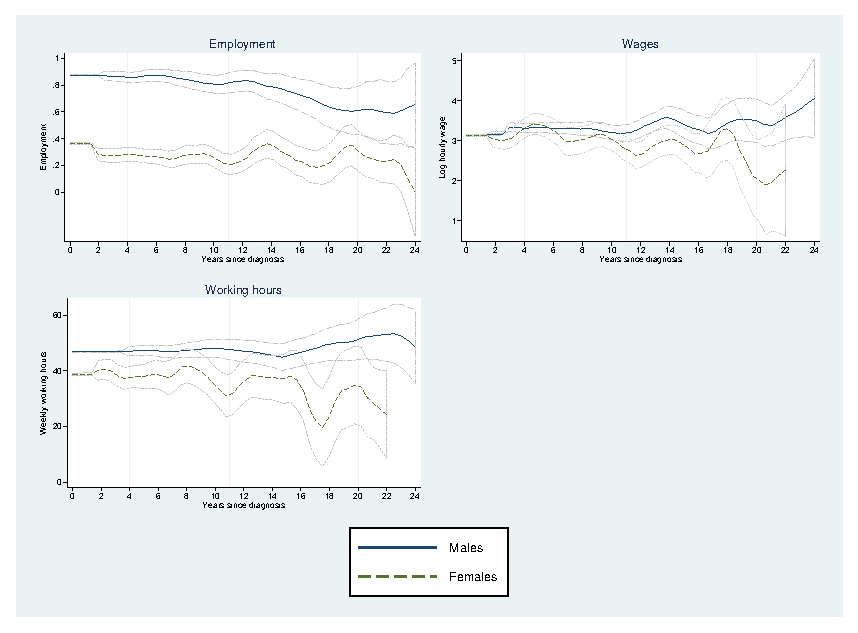
\includegraphics[width=\linewidth]{figures/lpoly_combined.eps}\\
		\footnotesize{\textit{Notes} The dashed lines show 95\% confidence intervals.}
	\end{center}
\end{figure}


\begin{figure}[h!]
	\caption{\label{fig:kdens_inconsistency_hba1c}Kernel density of HbA1c values for those with one inconsistent and two inconsistent reports.}%
	\begin{center}
		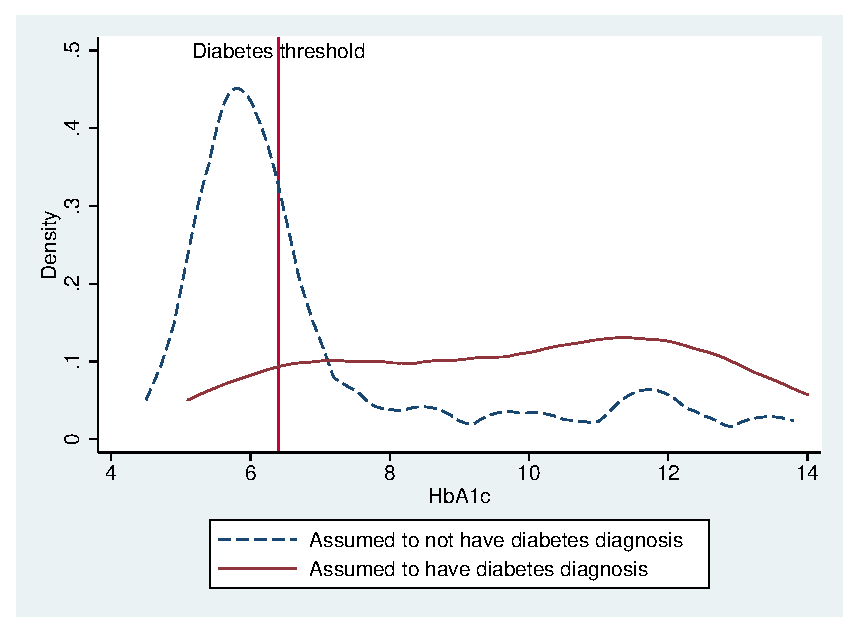
\includegraphics[width=.7\linewidth]{figures/kdensity_hba1c_inconsist.eps}\\
	\end{center}
\end{figure}

\end{document}

